\documentclass[tikz,border=8pt]{standalone}
\usetikzlibrary{arrows.meta,positioning}
\begin{document}
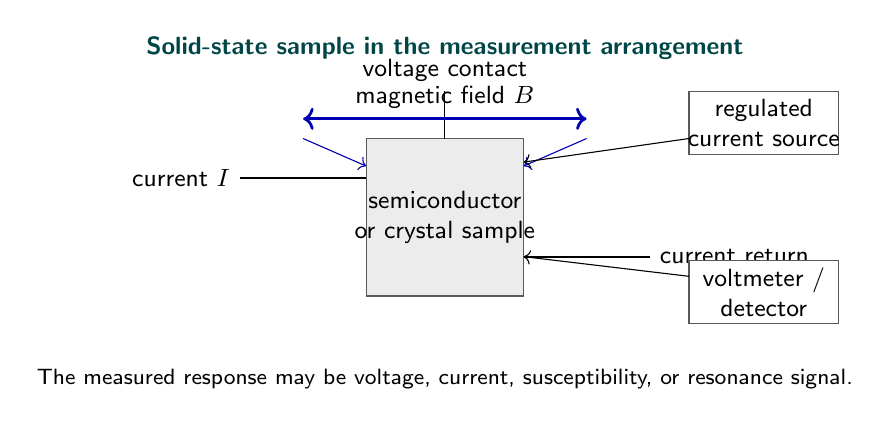
\begin{tikzpicture}[font=\sffamily\small]
\node[font=\sffamily\bfseries\small,text=teal!55!black] at (0,4.15) {Solid-state sample in the measurement arrangement};
\draw[fill=gray!15,draw=black!65] (-1.0,1.0) rectangle (1.0,3.0);
\node[align=center] at (0,2) {semiconductor\\or crystal sample};
\draw[thick] (-1,2.5)--(-2.6,2.5) node[left] {current $I$};
\draw[thick] (1,1.5)--(2.6,1.5) node[right] {current return};
\draw (0,3) -- (0,3.6) node[above] {voltage contact};
\draw[<->,blue!70!black,line width=1pt] (-1.8,3.25)--(1.8,3.25) node[midway,above,black] {magnetic field $B$};
\draw[->,blue!70!black] (-1.8,3.0)--(-1.0,2.65); \draw[->,blue!70!black] (1.8,3.0)--(1.0,2.65);
\draw[fill=white,draw=black!65] (3.1,2.8) rectangle (5.0,3.6);
\node[align=center] at (4.05,3.2) {regulated\\current source};
\draw[->] (3.1,3.0)--(1.0,2.7);
\draw[fill=white,draw=black!65] (3.1,.65) rectangle (5.0,1.45);
\node[align=center] at (4.05,1.05) {voltmeter /\\detector};
\draw[->] (3.1,1.25)--(1.0,1.5);
\node[font=\sffamily\footnotesize] at (0,-.05) {The measured response may be voltage, current, susceptibility, or resonance signal.};
\end{tikzpicture}
\end{document}
